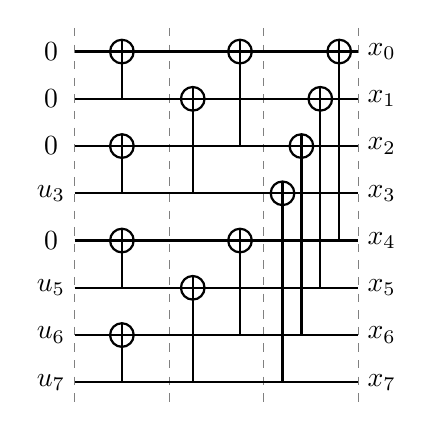
\begin{tikzpicture}[scale=.6, thick]

  \draw[very thin,gray,dashed] (1,.5) -- (1,-7.5);
  \draw[very thin,gray,dashed] (3,.5) -- (3,-7.5);
  \draw[very thin,gray,dashed] (5,.5) -- (5,-7.5);
  \draw[very thin,gray,dashed] (7,.5) -- (7,-7.5);

  %\node at (-.5,1) {layer};
  %\node at (1,1) {$0$};
  %\node at (3,1) {$1$};
  %\node at (5,1) {$2$};
  %\node at (7,1) {$3$};

  \node at (.5,0) {$0$};
  \node at (.5,-1) {$0$};
  \node at (.5,-2) {$0$};
  \node at (.5,-3) {$u_3$};
  \node at (.5,-4) {$0$};
  \node at (.5,-5) {$u_5$};
  \node at (.5,-6) {$u_6$};
  \node at (.5,-7) {$u_7$};

  \draw (1,0) -- (7,0);
  \draw (1,-1) -- (7,-1);
  \draw (1,-2) -- (7,-2);
  \draw (1,-3) -- (7,-3);
  \draw (1,-4) -- (7,-4);
  \draw (1,-5) -- (7,-5);
  \draw (1,-6) -- (7,-6);
  \draw (1,-7) -- (7,-7);

  \draw (2,0) circle [radius=.25];
  \draw (2,-2) circle [radius=.25];
  \draw (2,-4) circle [radius=.25];
  \draw (2,-6) circle [radius=.25];
  
  \draw (2,-1) -- ++(0,1.25);
  \draw (2,-3) -- ++(0,1.25);
  \draw (2,-5) -- ++(0,1.25);
  \draw (2,-7) -- ++(0,1.25);
  
  \draw (4.5,0) circle [radius=.25];
  \draw (3.5,-1) circle [radius=.25];
  \draw (4.5,-4) circle [radius=.25];
  \draw (3.5,-5) circle [radius=.25];

  \draw (4.5,-2) -- ++(0,2.25);
  \draw (3.5,-3) -- ++(0,2.25);
  \draw (4.5,-6) -- ++(0,2.25);
  \draw (3.5,-7) -- ++(0,2.25);

  \draw (6.6,0) circle [radius=.25];
  \draw (6.2,-1) circle [radius=.25];
  \draw (5.8,-2) circle [radius=.25];
  \draw (5.4,-3) circle [radius=.25];

  \draw (6.6,-4) -- ++(0,4.25);
  \draw (6.2,-5) -- ++(0,4.25);
  \draw (5.8,-6) -- ++(0,4.25);
  \draw (5.4,-7) -- ++(0,4.25);

  \node at (7.5,0) {$x_0$};
  \node at (7.5,-1) {$x_1$};
  \node at (7.5,-2) {$x_2$};
  \node at (7.5,-3) {$x_3$};
  \node at (7.5,-4) {$x_4$};
  \node at (7.5,-5) {$x_5$};
  \node at (7.5,-6) {$x_6$};
  \node at (7.5,-7) {$x_7$};

\end{tikzpicture}